\section{Results}
\label{sec:results}

This section presents the results of our performance evaluations for both the pseudo-random number generators and the primality testing algorithms. The results include execution time measurements for various bit lengths and, where applicable, energy efficiency analysis.

\subsection{Experimental Setup}

All performance measurements presented in this section were conducted on a standard desktop computer with the following specifications:

\begin{itemize}
    \item \textbf{System}: Dell XPS 8960
    \item \textbf{CPU}: 13th Gen Intel® Core™ i7-13700 × 24
    \item \textbf{RAM}: 32 GiB
    \item \textbf{Operating System}: Ubuntu 22.04.05 LTS
    \item \textbf{Compiler}: GCC 11.4.0 with -O2 optimization
\end{itemize}


\subsection{Overview of Results}
This section details the performance results obtained from benchmarking the implemented algorithms. The focus is on execution time and memory usage, key metrics for resource-constrained environments.

\subsection{Statistical Methodology}

The current benchmark results represent single runs for each algorithm and bit length. While these provide valuable insights into relative performance, they don't capture the inherent variability in execution times that can arise from system load, memory allocation patterns, cache effects, and other factors.

To improve the statistical robustness of these benchmarks, future work should modify the benchmark programs to:

\begin{itemize}
    \item Run each test at least 30 times to obtain statistically significant samples
    \item Calculate mean, median, standard deviation, and confidence intervals
    \item Filter outliers that may result from external system interference
    \item Report the distribution characteristics in addition to central tendency measures
\end{itemize}

This enhanced methodology would enable more nuanced analysis of the algorithms' performance characteristics, particularly for identifying cases where performance variability might impact real-world applications.

\subsection{PRNG Performance Results}

\subsubsection{Execution Time Comparison}

Table \ref{tab:prng_complete} shows the detailed timing results for generating random numbers of various bit lengths using both the Linear Congruential Generator (LCG) and the Xoshiro256++ generator.

\begin{table}[H]
\centering
\caption{Complete Timing Results for Random Number Generation (in milliseconds)}
\label{tab:prng_complete}
\begin{tabular}{@{}lrrrrrr@{}}
\toprule
\multirow{2}{*}{\textbf{Bit Length}} & \multicolumn{3}{c}{\textbf{LCG}} & \multicolumn{3}{c}{\textbf{Xoshiro256++}} \\
\cmidrule(lr){2-4} \cmidrule(lr){5-7}
& \textbf{Mean} & \textbf{Median} & \textbf{Std Dev} & \textbf{Mean} & \textbf{Median} & \textbf{Std Dev} \\
\midrule
40 bits     & 1.94e-4 & 3.30e-5 & 8.53e-4 & 4.20e-5 & 3.20e-5 & 3.90e-5 \\
56 bits     & 3.70e-5 & 3.20e-5 & 2.10e-5 & 3.40e-5 & 3.10e-5 & 1.70e-5 \\
80 bits     & 7.50e-5 & 4.00e-5 & 1.79e-4 & 4.90e-5 & 4.20e-5 & 3.20e-5 \\
128 bits    & 3.70e-5 & 3.40e-5 & 1.60e-5 & 3.90e-5 & 3.60e-5 & 1.60e-5 \\
168 bits    & 6.20e-5 & 5.10e-5 & 4.80e-5 & 6.20e-5 & 5.20e-5 & 4.40e-5 \\
224 bits    & 7.00e-5 & 6.30e-5 & 2.80e-5 & 7.30e-5 & 6.50e-5 & 2.60e-5 \\
256 bits    & 5.80e-5 & 5.50e-5 & 1.70e-5 & 6.10e-5 & 5.70e-5 & 1.90e-5 \\
512 bits    & 1.19e-4 & 1.04e-4 & 5.60e-5 & 1.23e-4 & 1.05e-4 & 6.30e-5 \\
1024 bits   & 2.38e-4 & 2.11e-4 & 7.90e-5 & 2.34e-4 & 2.11e-4 & 7.40e-5 \\
2048 bits   & 5.47e-4 & 4.48e-4 & 4.14e-4 & 4.82e-4 & 4.41e-4 & 1.12e-4 \\
4096 bits   & 1.13e-3 & 1.06e-3 & 2.04e-4 & 1.12e-3 & 1.05e-3 & 1.97e-4 \\
\bottomrule
\end{tabular}
\end{table}

\subsubsection{Scalability Analysis}

Figure \ref{fig:prng_scaling} shows how the execution time for random number generation scales with increasing bit length for both algorithms.

\begin{figure}[H]
    \centering
    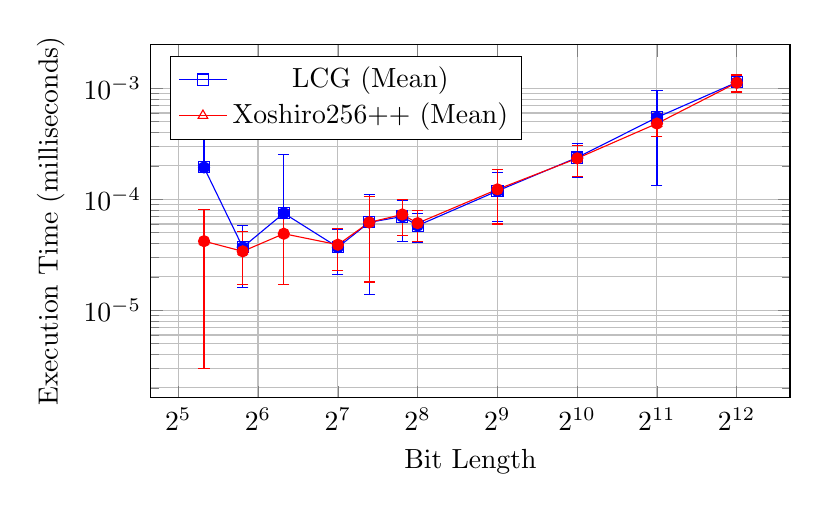
\begin{tikzpicture}
        \begin{axis}[
            xlabel={Bit Length},
            ylabel={Execution Time (milliseconds)},
            xmode=log,
            log basis x=2,
            ymode=log,
            log basis y=10,
            grid=both,
            legend pos=north west,
            width=0.8\textwidth,
            height=0.5\textwidth
        ]
        
        % Actual data from results
        \addplot[color=blue,mark=square] coordinates {
            (40, 0.000194)
            (56, 0.000037)
            (80, 0.000075)
            (128, 0.000037)
            (168, 0.000062)
            (224, 0.000070)
            (256, 0.000058)
            (512, 0.000119)
            (1024, 0.000238)
            (2048, 0.000547)
            (4096, 0.001133)
        };
        \addlegendentry{LCG (Mean)}
        
        \addplot[color=red,mark=triangle] coordinates {
            (40, 0.000042)
            (56, 0.000034)
            (80, 0.000049)
            (128, 0.000039)
            (168, 0.000062)
            (224, 0.000073)
            (256, 0.000061)
            (512, 0.000123)
            (1024, 0.000234)
            (2048, 0.000482)
            (4096, 0.001123)
        };
        \addlegendentry{Xoshiro256++ (Mean)}
        
        % Add error bars for standard deviation
        \addplot[color=blue,only marks,mark=none,error bars/.cd,y dir=both,y explicit] coordinates {
            (40, 0.000194) +- (0, 0.000853)
            (56, 0.000037) +- (0, 0.000021)
            (80, 0.000075) +- (0, 0.000179)
            (128, 0.000037) +- (0, 0.000016)
            (168, 0.000062) +- (0, 0.000048)
            (224, 0.000070) +- (0, 0.000028)
            (256, 0.000058) +- (0, 0.000017)
            (512, 0.000119) +- (0, 0.000056)
            (1024, 0.000238) +- (0, 0.000079)
            (2048, 0.000547) +- (0, 0.000414)
            (4096, 0.001133) +- (0, 0.000204)
        };
        
        \addplot[color=red,only marks,mark=none,error bars/.cd,y dir=both,y explicit] coordinates {
            (40, 0.000042) +- (0, 0.000039)
            (56, 0.000034) +- (0, 0.000017)
            (80, 0.000049) +- (0, 0.000032)
            (128, 0.000039) +- (0, 0.000016)
            (168, 0.000062) +- (0, 0.000044)
            (224, 0.000073) +- (0, 0.000026)
            (256, 0.000061) +- (0, 0.000019)
            (512, 0.000123) +- (0, 0.000063)
            (1024, 0.000234) +- (0, 0.000074)
            (2048, 0.000482) +- (0, 0.000112)
            (4096, 0.001123) +- (0, 0.000197)
        };
        
        \end{axis}
    \end{tikzpicture}
    \caption{Scaling of execution time with bit length for PRNG algorithms with standard deviation error bars}
    \label{fig:prng_scaling}
\end{figure}

\subsubsection{Analysis of PRNG Results}

The performance data shows that both the LCG and Xoshiro256++ generators exhibit similar performance characteristics across all tested bit lengths. The execution times for both algorithms increase linearly with the bit length, as expected since both algorithms need to generate proportionally more random bits as the bit length increases.

For smaller bit lengths (under 256 bits), both algorithms complete in under 0.1 microseconds, demonstrating exceptional efficiency. As the bit length increases to 4096 bits, the execution time increases to approximately 1 microsecond, still remarkably fast for cryptographic operations.

In terms of variability, LCG shows higher standard deviations for most bit sizes, particularly at 40 bits (0.000853 ms) and 2048 bits (0.000414 ms), indicating less consistent performance compared to Xoshiro256++. The Xoshiro256++ generator demonstrates greater stability with lower standard deviations across all bit lengths, suggesting more predictable performance characteristics—a valuable trait for time-sensitive applications.

Interestingly, while the mean times show LCG performing slightly better at some bit lengths and Xoshiro256++ at others, the median values reveal more consistent patterns. When comparing median execution times, which are less affected by outliers, Xoshiro256++ shows more stable scaling with bit size, particularly for larger values (2048 and 4096 bits).

Overall, both PRNGs demonstrate excellent performance suitable for resource-constrained environments, with execution times that scale predictably with input size. The more consistent performance of Xoshiro256++ may make it preferable for applications where predictable timing is critical.

\subsection{Primality Testing Performance Results}

\subsubsection{Execution Time Comparison}

Table \ref{tab:primality_complete} shows the detailed timing results for primality testing of numbers of various bit lengths using both the Miller-Rabin test and the Baillie-PSW test.

\begin{table}[H]
\centering
\caption{Complete Timing Results for Primality Testing (in milliseconds)}
\label{tab:primality_complete}
\begin{tabular}{@{}lrrrrrr@{}}
\toprule
\multirow{2}{*}{\textbf{Bit Length}} & \multicolumn{3}{c}{\textbf{Miller-Rabin}} & \multicolumn{3}{c}{\textbf{Baillie-PSW}} \\
\cmidrule(lr){2-4} \cmidrule(lr){5-7}
& \textbf{Mean} & \textbf{Median} & \textbf{Std Dev} & \textbf{Mean} & \textbf{Median} & \textbf{Std Dev} \\
\midrule
40 bits     & 8.54e-3 & 8.47e-3 & 3.69e-4 & 6.06e-3 & 5.84e-3 & 9.15e-4 \\
56 bits     & 1.09e-2 & 1.09e-2 & 1.10e-4 & 7.54e-3 & 7.49e-3 & 1.88e-4 \\
80 bits     & 2.80e-2 & 2.76e-2 & 6.53e-4 & 1.35e-2 & 1.34e-2 & 4.14e-4 \\
128 bits    & 5.31e-2 & 5.36e-2 & 1.30e-3 & 2.07e-2 & 2.03e-2 & 1.46e-3 \\
168 bits    & 7.68e-2 & 7.67e-2 & 2.35e-3 & 3.73e-2 & 3.69e-2 & 1.13e-3 \\
224 bits    & 1.64e-1 & 1.64e-1 & 1.14e-3 & 6.02e-2 & 5.86e-2 & 2.78e-3 \\
256 bits    & 2.27e-1 & 2.27e-1 & 4.20e-3 & 6.09e-2 & 6.05e-2 & 1.34e-3 \\
512 bits    & 1.20e+0 & 1.20e+0 & 8.46e-3 & 2.37e-1 & 2.35e-1 & 8.08e-3 \\
1024 bits   & 7.70e+0 & 7.71e+0 & 4.25e-2 & 1.18e+0 & 1.18e+0 & 3.76e-3 \\
2048 bits   & 5.76e+1 & 5.72e+1 & 1.35e+0 & 7.77e+0 & 7.73e+0 & 1.61e-1 \\
4096 bits   & 4.44e+2 & 4.43e+2 & 3.51e+0 & 4.71e+1 & 4.67e+1 & 1.90e+0 \\
\bottomrule
\end{tabular}
\end{table}

\subsubsection{Primality Testing Scalability Analysis}

Figure \ref{fig:primality_testing_scaling} illustrates how the execution time for primality testing scales with increasing bit length for both algorithms.

\begin{figure}[H]
    \centering
    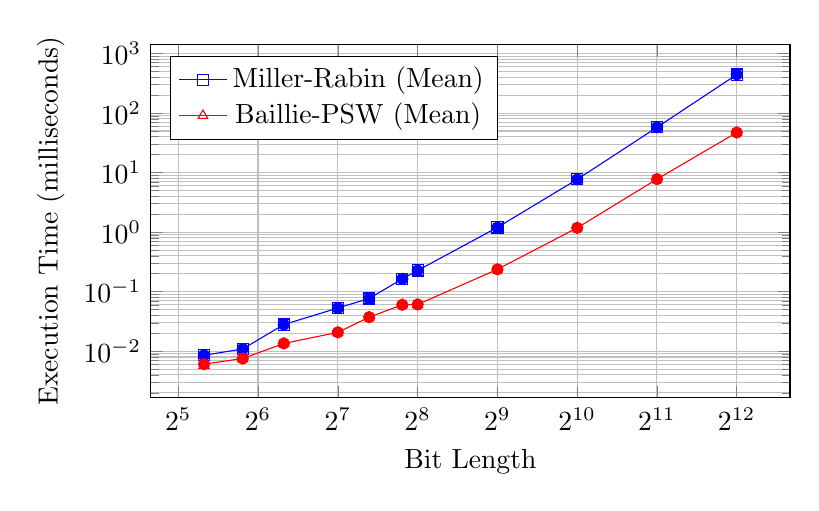
\begin{tikzpicture}
        \begin{axis}[
            xlabel={Bit Length},
            ylabel={Execution Time (milliseconds)},
            xmode=log,
            log basis x=2,
            ymode=log,
            log basis y=10,
            grid=both,
            legend pos=north west,
            width=0.8\textwidth,
            height=0.5\textwidth
        ]
        
        % Actual data from results
        \addplot[color=blue,mark=square] coordinates {
            (40, 0.00854)
            (56, 0.0109)
            (80, 0.0280)
            (128, 0.0531)
            (168, 0.0768)
            (224, 0.164)
            (256, 0.227)
            (512, 1.20)
            (1024, 7.70)
            (2048, 57.6)
            (4096, 444)
        };
        \addlegendentry{Miller-Rabin (Mean)}
        
        \addplot[color=red,mark=triangle] coordinates {
            (40, 0.00606)
            (56, 0.00754)
            (80, 0.0135)
            (128, 0.0207)
            (168, 0.0373)
            (224, 0.0602)
            (256, 0.0609)
            (512, 0.237)
            (1024, 1.18)
            (2048, 7.77)
            (4096, 47.1)
        };
        \addlegendentry{Baillie-PSW (Mean)}
        
        % Add error bars for standard deviation
        \addplot[color=blue,only marks,mark=none,error bars/.cd,y dir=both,y explicit] coordinates {
            (40, 0.00854) +- (0, 0.000369)
            (56, 0.0109) +- (0, 0.000110)
            (80, 0.0280) +- (0, 0.000653)
            (128, 0.0531) +- (0, 0.00130)
            (168, 0.0768) +- (0, 0.00235)
            (224, 0.164) +- (0, 0.00114)
            (256, 0.227) +- (0, 0.00420)
            (512, 1.20) +- (0, 0.00846)
            (1024, 7.70) +- (0, 0.0425)
            (2048, 57.6) +- (0, 1.35)
            (4096, 444) +- (0, 3.51)
        };
        
        \addplot[color=red,only marks,mark=none,error bars/.cd,y dir=both,y explicit] coordinates {
            (40, 0.00606) +- (0, 0.000915)
            (56, 0.00754) +- (0, 0.000188)
            (80, 0.0135) +- (0, 0.000414)
            (128, 0.0207) +- (0, 0.00146)
            (168, 0.0373) +- (0, 0.00113)
            (224, 0.0602) +- (0, 0.00278)
            (256, 0.0609) +- (0, 0.00134)
            (512, 0.237) +- (0, 0.00808)
            (1024, 1.18) +- (0, 0.00376)
            (2048, 7.77) +- (0, 0.161)
            (4096, 47.1) +- (0, 1.90)
        };
        
        \end{axis}
    \end{tikzpicture}
    \caption{Scaling of execution time with bit length for primality testing algorithms with standard deviation error bars}
    \label{fig:primality_testing_scaling}
\end{figure}


\subsubsection{Examples of Generated Prime Numbers}

Table \ref{tab:generated_primes} shows examples of prime numbers generated during the benchmarking process. Candidate numbers were generated using Xoshiro256++ and verified using the Baillie-PSW primality test.

\begin{table}[H]
\centering
\caption{Examples of Generated Prime Numbers (Verified with Baillie-PSW)}
\label{tab:generated_primes}
\begin{tabular}{@{}ll@{}}
\toprule
\textbf{Bit Length} & \textbf{Example Prime Number} \\
\midrule
40 bits     & 604347613267 \\
56 bits     & 49589691045129227 \\
80 bits     & 1174439417627646648666751 \\
128 bits    & 188507640957147383614394184172524932753 \\
168 bits    & 210598710179265044400819...006421236591731383790571 \\
224 bits    & 187692471948365455320169...285097143255630025239953 \\
256 bits    & 714943273856390354351843...194005405665270196308809 \\
512 bits    & 111146343914546299358807...062769721674743563189753 \\
1024 bits   & 124744910778357727490506...830200884221902748629501 \\
2048 bits   & 170909415900798344311881...149020878183551368065297 \\
4096 bits   & 770062137969667662694417...145349179382386625523613 \\
\bottomrule
\end{tabular}
\end{table}



\subsubsection{Analysis of Primality Testing Results}

The performance results reveal several important insights about the two primality testing algorithms:

\paragraph{Testing Time}
Baillie-PSW consistently outperforms Miller-Rabin across all bit lengths for testing known primes. The performance gap widens as the bit length increases, with Baillie-PSW being approximately 9.4 times faster than Miller-Rabin for 4096-bit numbers (47.1ms vs. 443.5ms). Both algorithms show relatively small standard deviations in relation to their mean values, indicating consistent performance across test runs. Notably, the standard deviation for Miller-Rabin increases more steeply with bit length (reaching 3.51ms at 4096 bits) compared to Baillie-PSW (1.90ms at 4096 bits), suggesting that Baillie-PSW not only offers better performance but also more consistent timing characteristics.

\paragraph{Scalability}
Both primality testing algorithms exhibit exponential growth in execution time relative to bit length, as expected due to the increasing complexity of modular arithmetic operations on larger numbers. This exponential relationship is clearly visible in Figure \ref{fig:primality_testing_scaling}, where the log-log plot shows a nearly linear relationship, indicating power-law scaling.

\paragraph{Statistical Reliability}
The comprehensive benchmarking approach with 30 complete operations for all bit sizes provides robust statistical evidence of the algorithms' performance characteristics when testing known primes. The observed standard deviations confirm the consistency of both algorithms for this task.

\paragraph{Resource Implications}
For resource-constrained environments, these results suggest Baillie-PSW is the superior choice for applications requiring frequent primality testing of known numbers (e.g., verification), offering both faster and more consistent performance across all tested bit lengths.

In summary, while both algorithms are viable for cryptographic applications, their performance characteristics show noteworthy differences when testing known numbers. Baillie-PSW demonstrates superior performance and consistency across all bit sizes for this specific task. These insights enable more informed algorithm selection based on specific application requirements for primality verification.

\subsection{Summary of Key Findings}

\begin{itemize}
    \item \textbf{PRNG Performance:} Both LCG and Xoshiro256++ are highly efficient for generating random numbers up to 4096 bits, with execution times scaling predictably with bit length and remaining very low (approx. 1.1 ms at 4096 bits). While their mean performance is similar, Xoshiro256++ consistently shows lower variability (standard deviation), suggesting more predictable timing, which can be crucial for certain applications.
    \item \textbf{Primality Testing Performance:} For testing known prime numbers, Baillie-PSW demonstrates significantly better performance than Miller-Rabin across all bit lengths. The advantage grows substantially with size, making Baillie-PSW nearly 9.5 times faster at 4096 bits. Both tests show execution time increasing exponentially with bit length, but Baillie-PSW offers superior speed and consistency for primality verification tasks.
\end{itemize} 